
%%%%%%%%%%%%%%%%%%%%%%%%%%%%%%%%%%%%%%%%%%%%%%%%%%%%%%%%%%%%%%%%%%%%%%%%%%%%%
\section{Code tests}
\label{sec.tests}

%%%%%%%%%%%%%%%%%%%%%%%%%%%%%%%%%%%%%%%%%%%%%%%%%%%%%%%%%%%%%%%%%%%%%%%%%%%%%
\subsection{Verifying and validating the \enzo\ code}
\label{sec.tests.vandv}

\red{(Britton)} Description of test suite and test runner.

\red{(Brian)} Refer to all code comparisons that Enzo has been part of.

%%%%%%%%%%%%%%%%%%%%%%%%%%%%%%%%%%%%%%%%%%%%%%%%%%%%%%%%%%%%%%%%%%%%%%%%%%%%%
\subsection{Representative test problems}
\label{sec.tests.problems}

General structure for each test problem:  Outline how the test problem is constructed (initial and boundary conditions), 
the analytical solution, why we have in the paper (what does it break, or what flaw does it expose (not in enzo of course)),
a plot showing how well enzo solves said test problem, and a brief description of the plot and how awesome enzo is.

%%%%%%%%%%%%%%%%%%%%%%%%%%%%%%%%%%%%%%%
\subsubsection{Sod Shock Tube}
\label{sec.tests.sodshock}
\red{(Greg)}
Problem type 1.  AMR version.  Tests the hydro.
This is also problem 7.2 in the FLASH method paper.

%%%%%%%%%%%%%%%%%%%%%%%%%%%%%%%%%%%%%%%
\subsubsection{Wave pool}
\label{sec.tests.wavepool}
\red{(Greg)}
Problem type 2, with AMR.  Tests reflections of waves at grid boundaries.

%%%%%%%%%%%%%%%%%%%%%%%%%%%%%%%%%%%%%%%
\subsubsection{Shock pool}
\label{sec.tests.shockpool}
\red{(Greg)}
Problem type 3, with AMR.  Tests passage of shock through a refinement boundary.

%%%%%%%%%%%%%%%%%%%%%%%%%%%%%%%%%%%%%%%
\subsubsection{Double mach reflection}
\label{sec.tests.doublemach}
\red{(Brian)}
Problem type 4.  This is one of Alexei's test problems.  Tests
boundary conditions in hydro.

%%%%%%%%%%%%%%%%%%%%%%%%%%%%%%%%%%%%%%%
\subsubsection{Sedov Explosion}
\label{sec.tests.sedov}
\red{(Elizabeth)}
Problem type 7.  One of Alexei's test problems.  
Also problem 7.4 in the FLASH method paper.
This tests the hydro in the strong-shock limit.

%%%%%%%%%%%%%%%%%%%%%%%%%%%%%%%%%%%%%%%
\subsubsection{Point source gravity test}
\label{sec.test.gravitypointsource}
\red{(Greg)}
This is the TestGravity (problem 23) test problem.  It tests gravity around a point source, using fixed AMR.

%%%%%%%%%%%%%%%%%%%%%%%%%%%%%%%%%%%%%%%
\subsubsection{Orbit Test}
\label{sec.test.testorbit}
\red{(Greg)}
This is the TestOrbit problem (problem 29 for GB).  This tests gravity and particle integration (no hydro).

%%%%%%%%%%%%%%%%%%%%%%%%%%%%%%%%%%%%%%%
\subsubsection{Self-Similar infall test}
\label{sec.tests.infall}
\red{(Greg)}
Problem type 24.  This is a test based on Bertschinger's 1985 3D self-similar infall
solution, and tests gravity + hydro.

%%%%%%%%%%%%%%%%%%%%%%%%%%%%%%%%%%%%%%%
\subsubsection{Zel`Dovich Pancake}
\label{sec.tests.pancake}
\red{(Brian)}
Problem type 20, unigrid and AMR both.  Tests gravity + hydro.

%%%%%%%%%%%%%%%%%%%%%%%%%%%%%%%%%%%%%%%
\subsubsection{Cosmology simulations}
\label{sec.tests.}
\red{(Brian)}
Talk about cosmology code comparisons, where Enzo is good/weak.

%%%%%%%%%%%%%%%%%%%%%%%%%%%%%%%%%%%%%%%
\subsubsection{MHD: Orszag-Tang Vortex}
\label{sec.tests.mhd}
Figure \ref{fig.orszag} shows the Orszag-Tang vortex problem, a typical test
problem for MHD \citep{Orszag79}.  The left panel shows the MHD-CT result, while
the right panel shows the Dedner result.  This test shows that small scale structure
can be generated in MHD from large scale initial perturbations.  
The test begins 
with uniform density, $\rho_0=25/36 \pi$ and pressure, $P_0=5/12 \pi$.  There is
a single rotational mode in the velocity, and two in the magnetic field: 
${\bf v}_0 $ = (-sin(2$\pi$ y) $ \hat{x}$ , sin(2$\pi$ x) $\hat{y}$),
${\bf B}_0$  =  (-sin(2 $\pi$ y) $ \hat{x},$ sin( 4 $\pi$ x )$\hat{y}$).  The
simulation is evolved to t=0.48.  One can see that the structures are accurately
represented as compared to, for instance, \citet{Toth00}, and that the
resolution of shocks is comparable in both methods.  

{\emph Dave's note:  I'll probably play around with these results in future
versions.}

\begin{figure}
\begin{center}
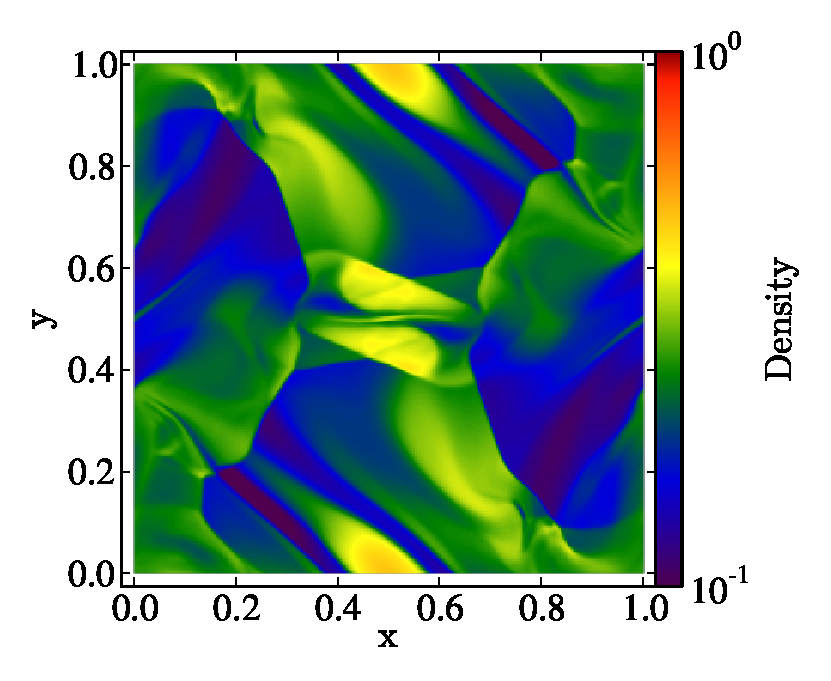
\includegraphics[width=0.4\textwidth]{figures/MHDCT_OrszagTang_Density.eps}
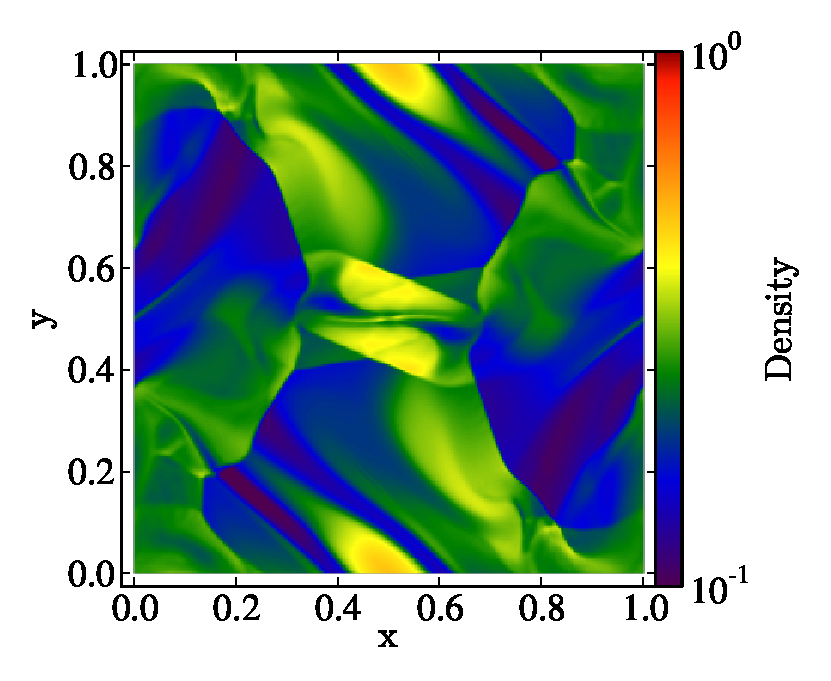
\includegraphics[width=0.4\textwidth]{figures/MHDDedner_OrszagTang_Density.eps}
\caption{TANG}
\label{fig.orszag}
\end{center}
\end{figure}


%%%%%%%%%%%%%%%%%%%%%%%%%%%%%%%%%%%%%%%
\subsubsection{1-zone free-fall test}
\label{sec.tests.freefall}
\red{(Britton)}
One zone free fall test.  Tests cooling, chemistry.

%%%%%%%%%%%%%%%%%%%%%%%%%%%%%%%%%%%%%%%
\subsubsection{Photo-evaporation of a dense clump}
\label{sec.tests.raytracing}
\red{(John)}
Photo-evaporation of a dense clump.  Tests ray tracing, specifically
the shadowing effects of the clump, and the hydrodynamic response of
the clump.

%%%%%%%%%%%%%%%%%%%%%%%%%%%%%%%%%%%%%%%
\subsubsection{Representative FLD test}
\label{sec.tests.fld}
\red{(Dan)}
One test for the implicit FLD: best/hardest one.


